\documentclass[12pt]{article}

\title{On the quantum decomposition of the planet Mercury's orbit path using post-Newtonian gravitation}
\author{S. Halayka\footnote{sjhalayka@gmail.com}}
\date{\today\;\currenttime}

\usepackage{datetime}
\usepackage{listings}
\usepackage{cite}
\usepackage{xcolor}
\usepackage{graphicx}
\usepackage{setspace}
\usepackage{amsmath}
\usepackage{url}
\usepackage[margin=1 in]{geometry}

%\doublespace

%\usepackage[]{lineno}
%\linenumbers


\begin{document}



 
\maketitle

\begin{abstract}
By quantizing the kinematic and gravitational time dilation using various step sizes, one obtains a set of weighted orbit paths.
The precession associated with each weighted orbit path combines to provide the same answer as the classical analytical solution.
\end{abstract}





\section{Introduction}

In a previous paper \cite{halayka}, we introduced a method of numerical simulation for the four Solar System tests of general relativity, in particular the precession of Mercury's orbit.
There was a catch: one had to quantize the kinematic and gravitational time dilation by casting the relevant floating point variables from double-precision to single-precision.
A first, this was taken to be a bug, but after careful consideration, it turns out to be a feature of reality.
This paper will demonstrate how to decompose the orbit path of Mercury, to numerically obtain the relativistic orbit precession.

The C++ code for this paper is available.
It uses the Boost multiprecision floating point library, so that we may specify an arbitrary number of mantissa bits.


\section{Quantization of time dilation}

In this paper, we will be quantizing the kinematic and gravitational time dilation by casting them to a lesser-precision floating point number.

The non-exponent bit count $n$ includes the number of mantissa bits $m$, plus one sign bit.
We generally used $n = 100$, except for the kinematic and gravitational time dilation, which uses a lesser, various precision (e.g. $n = 24$).

For subnormal numbers such as those used here, the smallest step size that can be represented is $\epsilon = 2 \times 2^{-b}$, where $b$ is the largest exponent value (e.g. $2^7 - 1 = 127$ in single-precision floating point numbers, $2^{10} - 1 = 1023$ for doubles).
For instance, we use $1023$ where $n = 100$, and $127$ otherwise (e.g. where $n = 24$).

As for $m$, it governs how many places there are after the decimal point.

See Figs. 1 and 2.


\section{Steps in spacetime}

Where $\ell_s$ denotes the Sun's location at the origin, $\ell_o$ denotes the orbiter Mercury's location, and $\vec{d}$ denotes the direction vector that points from the orbiter toward the Sun:
\begin{equation}
\label{direction_vector}
\vec{d} = \ell_{s} - \ell_{o},	
\end{equation}
\begin{equation}
\label{direction_unit_vector}
\hat{d} = \frac{\vec{d}}{\lvert\lvert \vec{d} \rvert\rvert},
\end{equation}
the Newtonian acceleration vector is:
\begin{equation}
\label{newton}
\vec{g}_n = \frac{\hat{d} G M}{{\lvert\lvert \vec{d} \rvert\rvert}^2}.
\end{equation}

One parameter is closely related to the kinematic time dilation:
\begin{equation}
\label{eq_kinematic}
\alpha = 2 - \sqrt{1 - \frac{\lvert\lvert \vec{v}_{o}\rvert\rvert^2}{c^2}}.
\end{equation}
Another parameter is the gravitational time dilation from the Schwarzschild solution:
\begin{equation}
\label{eq_gravitational}
\beta = \sqrt{1 - \frac{R_{s}}{\lvert \lvert \vec{d} \rvert \rvert}}.
\end{equation}

Finally, the semi-implicit Euler integration for velocity and then location is:
\begin{align}
\label{eq_velocity}
\vec{v}_{o}(t + \delta_t) &= \vec{v}_{o}(t) + \delta_{t} \alpha \vec{g}_n, \\
\label{eq_position}
\ell_{o}(t + \delta_t) &= \ell_{o}(t) + \delta_{t} \beta \vec{v}_{o}(t + \delta_t).
\end{align}
Note that Newtonian gravity is the result where $\alpha = \beta = 1$.

See Figs. 3 and 4.





\section{Classical analytical calculation of Mercury's orbit precession}

The classical orbit precession is:
\begin{equation}
\label{delta_p}
\delta_{p} = \frac{6 \pi G M}{c^2 (1 - e^2) a} \left( \frac{1}{ \pi \times 180 \times 3600} \right) \left( \frac{365}{88} \times 100 \right) = 42.937
\end{equation}
arcseconds per Earth century, where $e = 0.2056$ is the eccentricity, and $a = 5.7909 \times 10^{10}$ is the semi-major axis.

See Fig. 5.


\section{Quantum path decomposition}

Here we report the precession angle $\delta_{p}$ in terms of arcseconds per Earth century, after one full orbit.
There is a highly visible pattern, which we shall point out.

We use an initial location that is $6.9817079 \times 10^{10}$ metres from the Sun (e.g. the aphelion).
We use various initial speeds.

Where initial speed is $25000$ metres per second, and the analytical solution is $103.7$:
\begin{center}
\begin{tabular}{| l | r |}
  \hline
Bits $n$ & Angle $\delta_{p}$ \\
\hline
\hline
20 & 17..04 \\
21 & 17.04 \\
22 & 17.04 \\
23 & 47.8 \\
24 & 38.95 \\
25 & 34.8 \\
26 & 34.96 \\
27 & 34.9 \\
28 & 35.07 \\
29 & 35.08 \\
30 & 35.06 \\
  \hline  
\end{tabular}
\end{center}
If we add bit counts 22, 23, and 24 together (e.g. $17.04 + 47.8 + 38.95$) we get $103.79$ arcseconds per Earth century.
All of the other bit counts have a weight of zero.

Where initial speed is $20000$ metres per second, and the analytical solution is $162.09$:
\begin{center}
\begin{tabular}{| l | r |}
  \hline
Bits $n$ & Angle $\delta_{p}$\\
\hline
\hline
21 & 27.86 \\
22 & 76.62 \\
23 & 52.9 \\
  \hline  
\end{tabular}
\end{center}
If we add bit counts 21, 22, and 23 together, we get $157.38$.

Where initial speed is $30000$ metres per second, and the analytical solution is $72.04$:
\begin{center}
\begin{tabular}{| l | r |}
  \hline
Bits $n$ & Angle $\delta_{p}$\\
\hline
\hline
23 & 46.45 \\
24 & 27.8 \\
  \hline  
\end{tabular}
\end{center}
If we add bit counts 23 and 24 together, we get $74.25$.

Where initial speed is $38858.47$ metres per second (e.g. the actual speed at aphelion), and the analytical solution is $42.9$:
\begin{center}
\begin{tabular}{| l | r |}
  \hline
Bits $n$ & Angle $\delta_{p}$ \\
\hline
\hline
24 & 46.8 \\
  \hline  
\end{tabular}
\end{center}
See Eq. \ref{delta_p}.
Note that a single-precision floating point number has $24$ mantissa and sign bits.

Where initial speed is $42500$ metres per second, and the analytical solution is $35.8$:
\begin{center}
\begin{tabular}{| l | r |}
  \hline
Bits $n$ & Angle $\delta_{p}$\\
\hline
\hline
26 & 51.7 \\
  \hline  
\end{tabular}
\end{center}
Obviously, this final solution's weight is less than $1$ (e.g. $(35.8 / 51.7) < 1$).




\section{Conclusion}

Here we have quantized the kinematic and gravitational time dilation.
The result is a set of weighted orbit paths that add up to provide the same answer as the classical analytical solution.





\begin{thebibliography}{9}


\bibitem{halayka} Halayka. On simulating the four Solar System tests of general relativity using two-parameter post-Newtonian gravitation with Euler integration. (2024)
\bibitem{misner} Misner et al. Gravitation. (1970)

\end{thebibliography}






\pagebreak



\begin{figure} 
\centering
\label{fig7}
  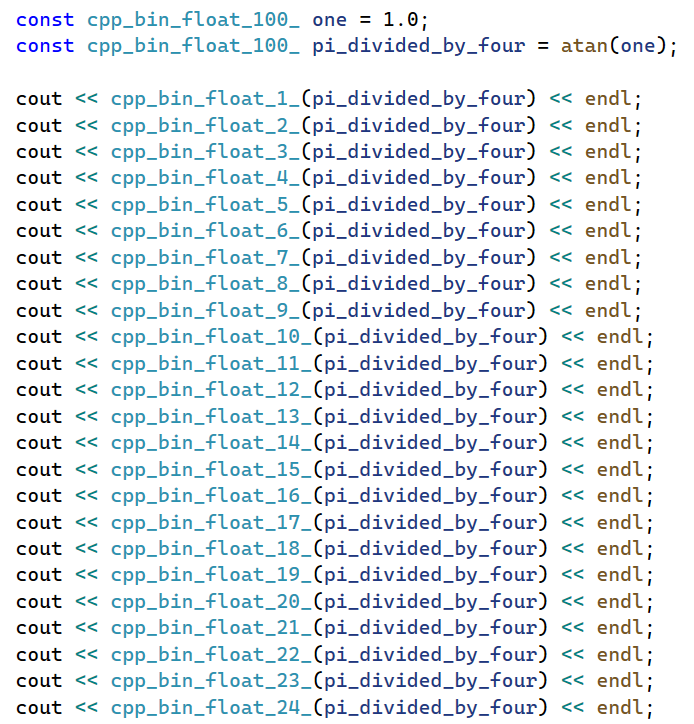
\includegraphics[width = 4 in]{code.png}
  \caption{
Code, showing the quantization of a constant $\pi/4$.
}
\end{figure}

\begin{figure} 
\centering
\label{fig7}
  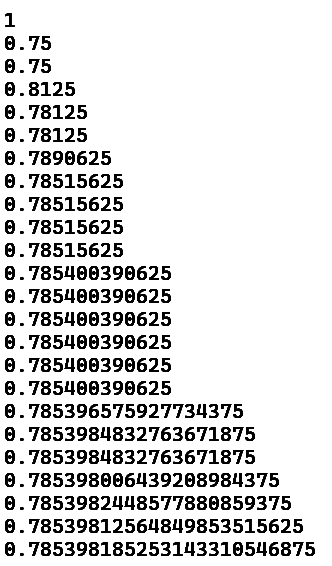
\includegraphics[width = 3 in]{code_output.png}
  \caption{
Output from the code.
}
\end{figure}







\begin{figure} 
\centering
\label{fig7}
  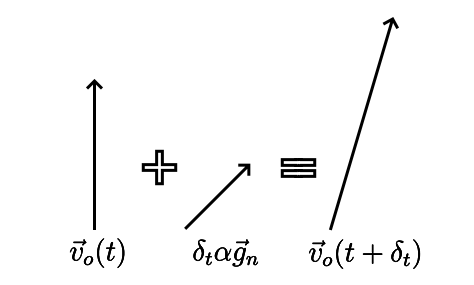
\includegraphics[width = 6 in]{velocity.png}
  \caption{
A diagram of the Euler integration of velocity.
}
\end{figure}

\begin{figure} 
\centering
\label{fig8}
  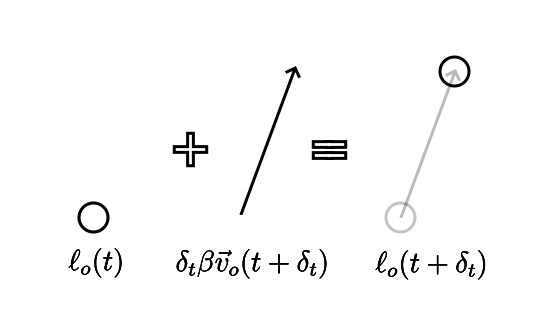
\includegraphics[width = 6 in]{location.png}
  \caption{
A diagram of the Euler integration of location.
}
\end{figure}



\begin{figure} 
\centering
\label{fig4}
  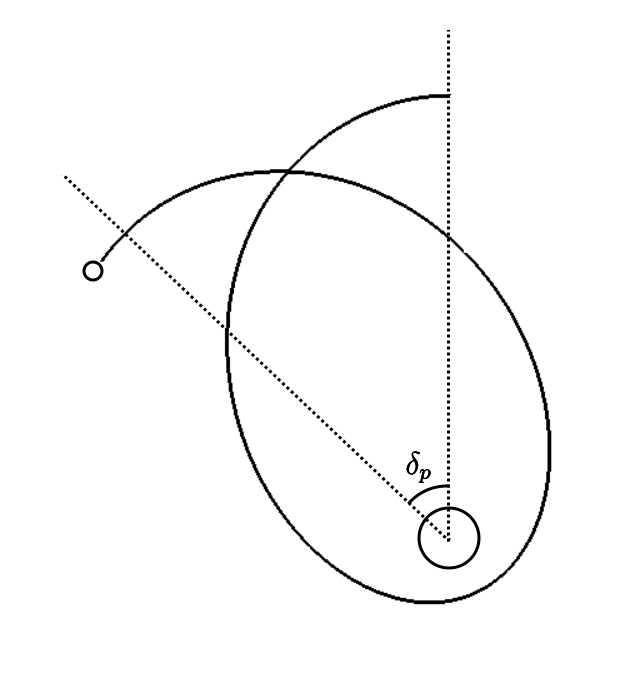
\includegraphics[width = 6 in]{precession.png}
  \caption{ A diagram showing precession, where the orbit does not quite form a closed ellipse.
}
\end{figure}





\end{document}









